
%%%%%%%%%%%%%%%%%%%%%%%%%%%%%%%%%%%%%%%%%%%%%%%%%%%%%%%%%%%%%%%%%%%%%%%%%%%%%%%%
%%%%%%%%%%%%%%%%%%%%%%%%%%%%%%%%%%%%%%%%%%%%%%%%%%%%%%%%%%%%%%%%%%%%%%%%%%%%%%%%
\section{Contagem de tempos correográficos}
\label{sec:TemposCoreograficos}
\index{Musicalidade!Tempos coreográficos}
Nesta seção presentamos e definimos o conceito de ``tempo coreográfico''.
Quando criamos uma coreografia, nós 
definimos uma distribuição de tempos na qual os movimentos serão executados;
para conseguir isto usamos como unidade de medida um tempo de referencia,
de modo que cada movimento na coreografia tem sua duração em referencia a este tempo.
\begin{definition}[Tempo coreográfico] 
\label{def:tempocoreografico}
é a unidade de medida básica com que os movimentos de uma coreografia são ordenados e distribuídos.
Um tempo coreográfico não precisa ter uma representação em segundos,
este dado só será relevante quando a coreografia seja encaixada numa música;
nesse caso: 
\begin{itemize}
\item Deverá ser indicada a equivalência entre os tempos coreográficos e musicais.
\item Também, deverá ser indicado a posição do primeiro tempo coreográfico em relação aos tempos musicais.
\end{itemize}
\end{definition}
Assim, a principio, os tempos coregráficos são bastante livres 
e seu uso e criação depende exclusivamente da imaginação do coreografo.


Para evitar confusões na leitura, aqui nós usaremos a abreviatura ``TC'' 
antes do número que indica o tempo coreográfico 
para diferenciar este na contagem do tempo musical.
Por exemplo quatro tempos coreográficos em sequência seriam escritos como: 
\{TC1, TC2, TC3, TC4\}.

De forma similar, para indicar um conjunto de 4 movimentos, 
sugerimos utilizar a abreviatura ``M''; de modo que quatro movimentos de uma coreografia 
ordenados em sequência seriam escritos como: 
\{M1, M2, M3, M4\}.

\begin{example}
Imaginemos que estamos criando o movimento chamado \hyperref[subsec:passo:romario]{\textbf{Romário}},
e decidimos iniciar ele da \hyperref[def:X-position]{\textbf{posição de X}}; 
percebemos então que faremos 6 movimentos,
de modo que o terceiro e sexto tem o tempo de espera dobrado, 
em relação aos demais movimentos que tem o mesmo tempo de espera apos serem executados.

Assim para descrever o Romário, antes de ser incrustado na música, 
poderíamos usar a seguinte sequencia de tempos coreográficos: \{TC1, TC2, TC3, TC5, TC6, TC7\},
que correspondem aos movimentos \{M1, M2, M3, M4, M5, M6\} da coreografia, respetivamente.

Para incrustar esta coreografia na música o único que precisamos indicar,
é que a coreografia inicia no tempo 2 do compasso (tempo fraco)
e que cada tempo coreográfico dura meio tempo musical.

A contagem de tempos coreográficos pode ser vista na primeira linha de texto na pauta mostrada na Figura \ref{fig:contagemtempocoreografico};
na segunda linha de texto da pauta podemos ver a contagem dos tempos musicais,
na qual vemos que o movimento todo da coreografia dura 4 tempos musicais.
\end{example}

\begin{figure}[!h]
    \centering
    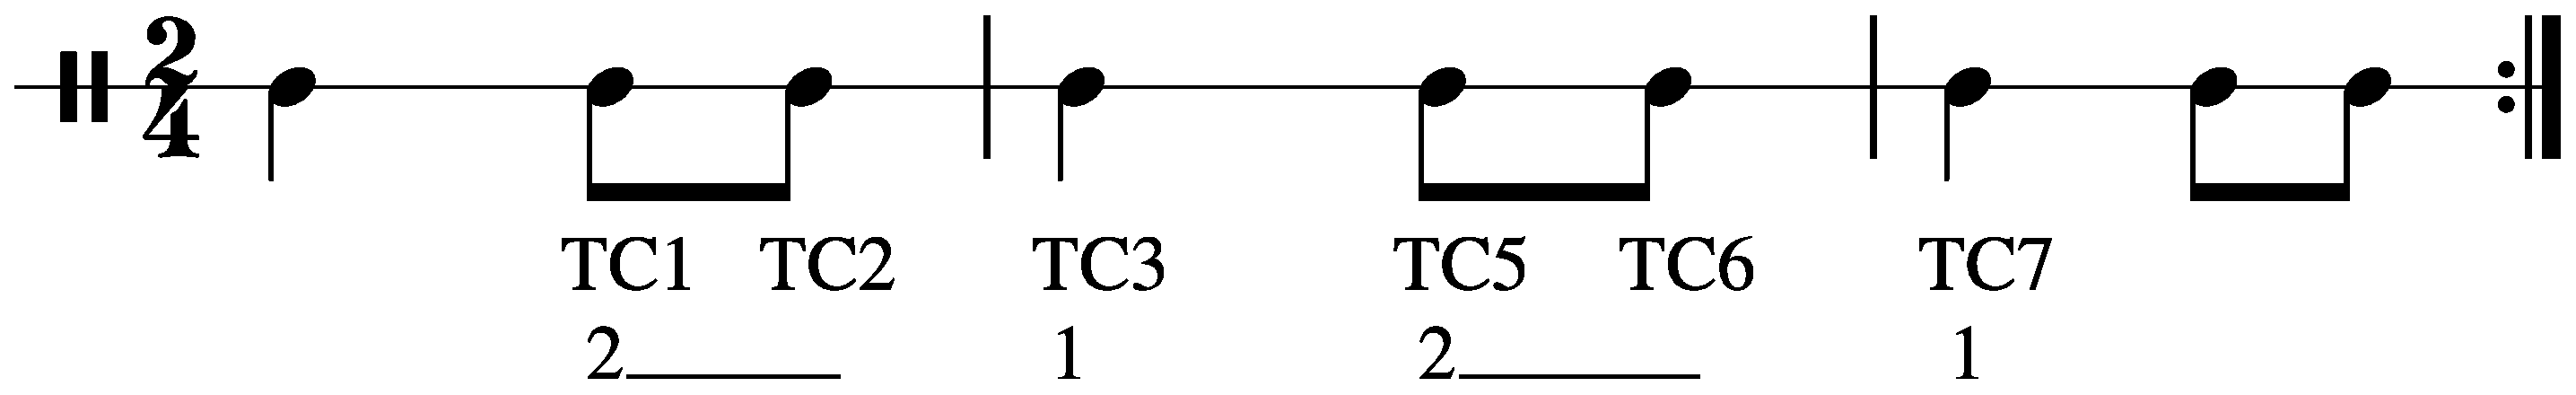
\includegraphics[width=\textwidth]{chapters/cap-musicalidade/abc-contagemtempocoreografico-1.eps}
\begin{comment}
\begin{abc}[name=abc-contagemtempocoreografico]
X: 1 % start of header
K: C stafflines=1 % scale: C major
M: 2/4 %meter - compasso
%Q:1/4=80
V:1 clef=perc stem=up %name="Pauta com clave de fá"   sname="Pauta com clave de fá"
[V:1] |: B2 B1 B1| B2 B1 B1 | B2 B1 B1 :|
w: ~ TC1 TC2 TC3 TC5 TC6 TC7 
w: ~ 2_ 1  2_ 1 ~  
\end{abc}
\end{comment}
    \vspace{-10pt}
    \caption{Contando tempos coregráficos.}
    \label{fig:contagemtempocoreografico}
\end{figure}

\begin{comment}
\begin{figure}[h]
\index{Tira}
    \centering
    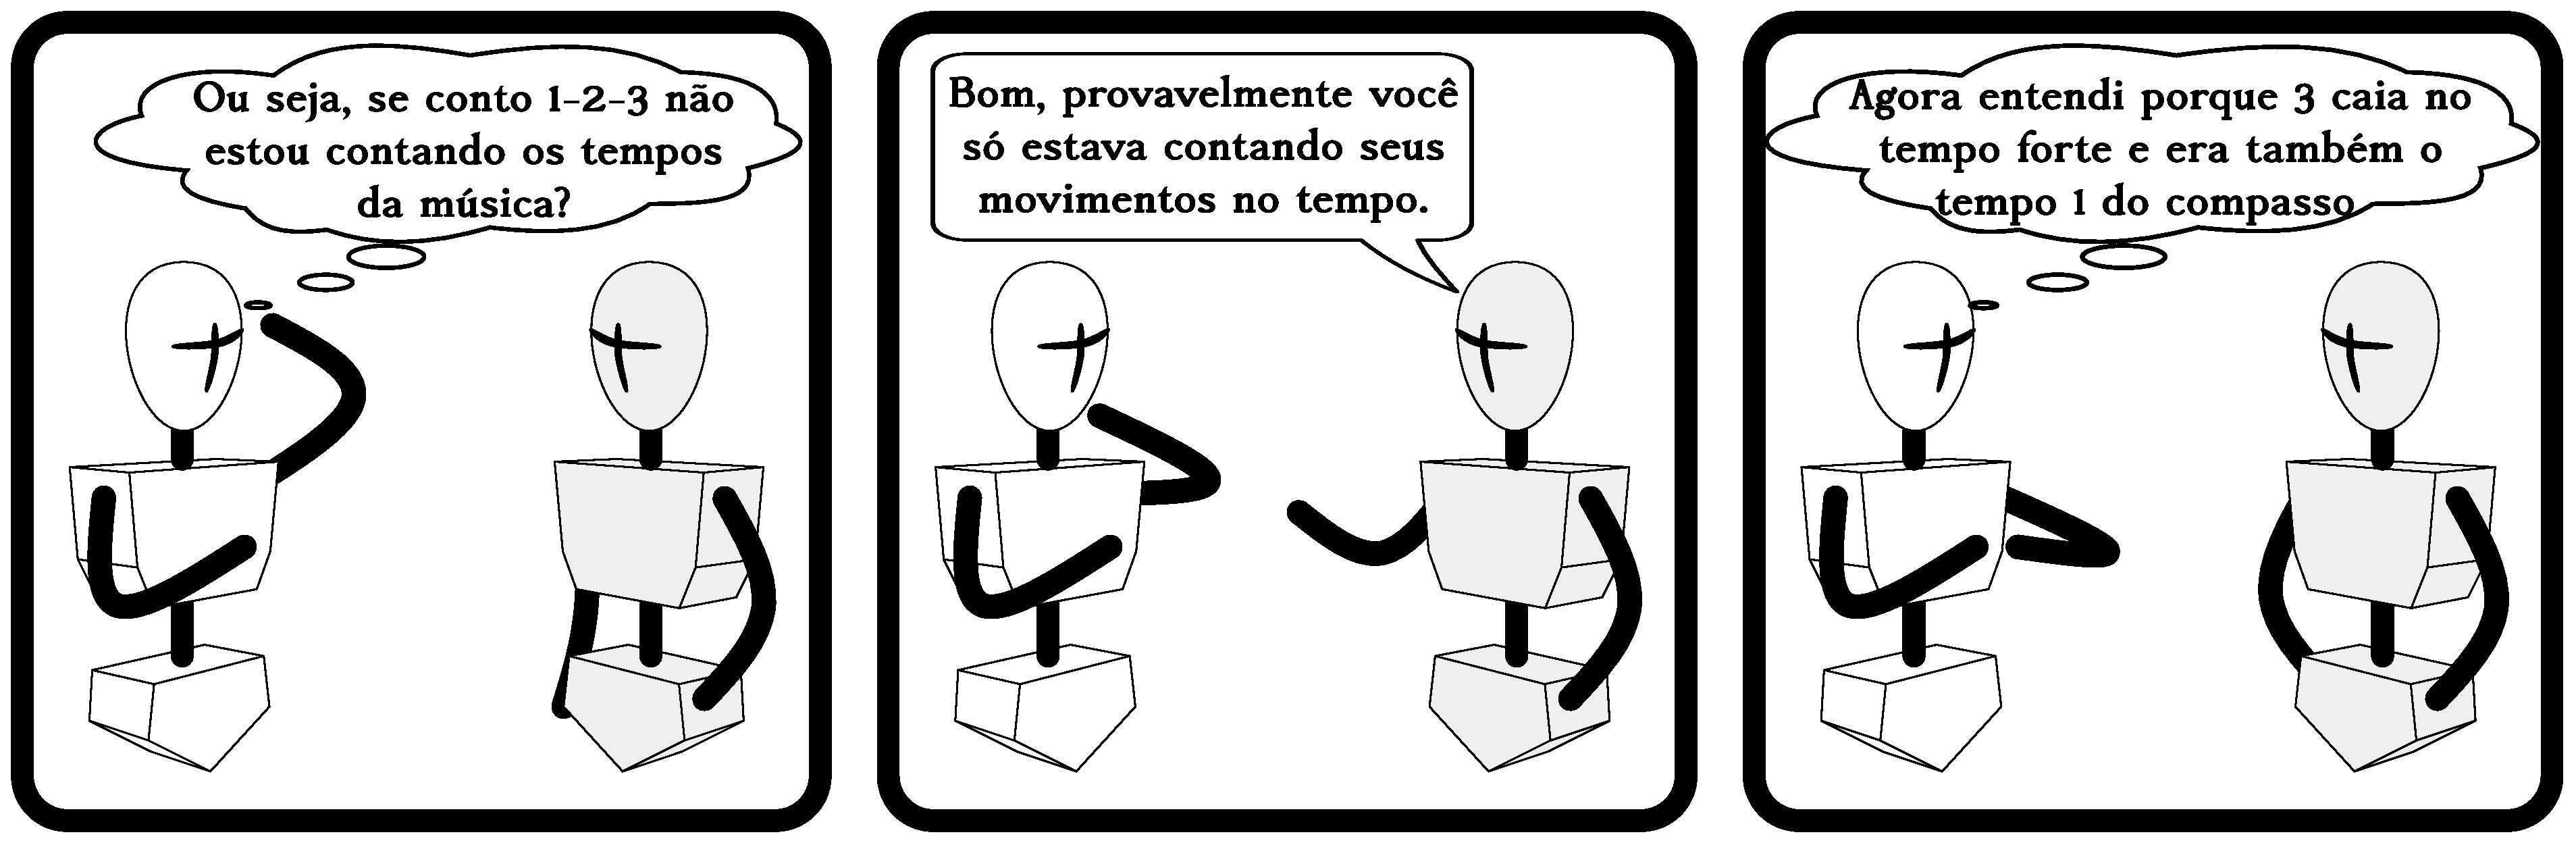
\includegraphics[width=\textwidth]{comic/tira-contagem.eps}
    %\caption{Contando tempos coregráficos.}
    %\label{fig:contagemtempocoreografico}
\end{figure}
\end{comment}
